\documentclass[xcolor=dvipsnames]{beamer}
\usepackage{graphicx}
\usepackage{xcolor}
\usepackage{tikz}
\usepackage{tikzscale}
\usetikzlibrary{positioning}
\usetikzlibrary{arrows.meta}
\usetikzlibrary{fit}
\usepackage{multicol}
\usepackage[export]{adjustbox}
\usepackage{tcolorbox}
\usepackage[overlay, absolute]{textpos}
\usepackage{fontspec}
\usepackage{appendixnumberbeamer}
\setsansfont[
ItalicFont=Roboto-LightItalic.ttf
]{Roboto Light}
\graphicspath{{fig/}}

% define themes
\usecolortheme{dolphin}

% change text to offblack
\definecolor{almostblack}{HTML}{262626}
\definecolor{gunmetal}{HTML}{5C5858}
\definecolor{pyred}{HTML}{F24532}
\definecolor{pyblue}{HTML}{2E7EBC}
\definecolor{pyorange}{HTML}{FEA862}
\definecolor{theme}{RGB}{90,122,163}

% set text color and theme color
\setbeamercolor{normal text}{fg=almostblack}
\usecolortheme[named=theme]{structure}

% macros
\newcommand{\trento}{T\raisebox{-0.3ex}{R}ENTo}

\makeatletter
\setbeamertemplate{frametitle}{
  \ifbeamercolorempty[bg]{frametitle}{}{\nointerlineskip}%
  \@tempdima=\textwidth%
  \advance\@tempdima by\beamer@leftmargin%
  \advance\@tempdima by\beamer@rightmargin%
  \begin{beamercolorbox}[sep=0.3cm,left,wd=\the\@tempdima]{
            frametitle}
    \vbox{}\vskip-2ex%
    \if@tempswa\else\csname beamer@fteleft\endcsname\fi%
    \strut\insertframetitle\strut\par%
    {%
      \ifx\insertframesubtitle\@empty%
      \else%
      {\usebeamerfont{framesubtitle}\usebeamercolor[fg]{
        framesubtitle}\insertframesubtitle\strut\par}%
      \fi
    }%
    \vskip.45ex%
    \hrule %height .6pt%
    \vskip-1.45ex%
    \if@tempswa\else\vskip-.3cm\fi%
  \end{beamercolorbox}%
}
\makeatother

% clean up footer
\beamertemplatenavigationsymbolsempty
\setbeamertemplate{footline}[text line]{
    \parbox{\linewidth}{\vspace*{-10pt}
            \raggedleft \color{gunmetal} 
            \bf J.\ Scott Moreland (Duke U.) 
            \quad \insertframenumber\,/\,\inserttotalframenumber}
}

%inner theme
\useinnertheme{rectangles}
\setbeamertemplate{itemize item}{
                   \raise.30ex\hbox{\vrule width .80ex height .80ex}}
\setbeamertemplate{itemize subitem}{
                   \raise.35ex\hbox{\vrule width .70ex height .70ex}}

\author{J.S.\ Moreland, J.E.\ Bernhard, S.A.\ Bass\\J.\ Liu, U.\ Heinz}
\date{May 25, 2016}

\begin{document}

\section{Title}

\usebackgroundtemplate{%
\tikz[overlay,remember picture] \node[opacity=0.4, at=(current page.center)] {
   \includegraphics[width=\paperwidth]{trento2}};
}

\frame[plain,noframenumbering]{
  \begin{tikzpicture}[remember picture,overlay]
    \coordinate (middle) at (current page.center);
    \def\sep{.028\paperwidth}
    \def\extra{.6em}
    \node[rectangle, fill=theme, align=center, anchor=center,
            yshift=2.75cm, fill opacity=0.08, text opacity=1] at (middle) {
      \color{theme} \Large
      Determining QGP initial conditions and medium\\
      \color{theme} \Large
      properties via Bayesian model-to-data analysis
    };
    \node[align=center, anchor=center, yshift=0.6 cm] at (middle) {
      \insertauthor \\[\extra]
      \small arXiv:1605.03954 \\ [\extra]
      Initial Stages~$\vert$~\insertdate
    };
    \node[align=center, anchor=center, yshift=-3.5 cm] at (middle) {
      \includegraphics[height=1.2cm]{qcdlogo} \hspace{0.2 cm} \hspace{0.2 cm}
      \includegraphics[height=1.cm]{ssgf} \vspace{0.2 cm} \\
      \scriptsize Funding provided by DOE Stewardship Science Graduate Fellowship
    };
  \end{tikzpicture}
}

\usebackgroundtemplate{}


\begin{frame}{Deconstructing initial condition models}
    \bigskip
    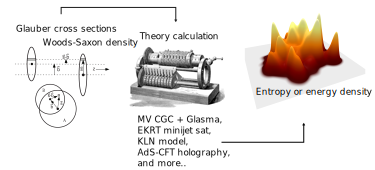
\includegraphics{deconstructing} \\
    \begin{itemize}
        \small
        \item Woods-Saxon, Glauber modeling aspects generally well accepted \\
        \smallskip
        \item Useful to separate cross sections and entropy deposition map, \\
              i.e.\ ~$dS/dy \sim f(T_A, T_B)$ where $T$ is the nuclear thickness.
              \emph{The mapping $f$ is a 2D surface.}
    \end{itemize}
\end{frame}


\begin{frame}{Parametrizing the initial conditions}
    \centering \vfill
    \begin{tcolorbox}[colback=theme!10, colframe=theme!0]
        \centering Generalized mean ansatz: \quad
                   $\displaystyle \frac{dS}{d^2r\, dy} \propto
                    \biggl(\frac{T_A^p + T_B^p}{2}\biggr)^{1/p}$
            \tikz[remember picture] \node[coordinate, above=5 pt] (d1) {};
    \end{tcolorbox}
    \smallskip
    \begin{columns}[T]
        \begin{column}{0.75\textwidth}
            \centering
            \includegraphics<1>[width=\textwidth]{thickness_band} 
            \includegraphics<2>[width=\textwidth]{thickness_arithmetic} 
            \includegraphics<3>[width=\textwidth]{thickness_geometric} 
            \includegraphics<4>[width=\textwidth]{thickness_harmonic} 
        \end{column}
        \begin{column}{0.25\textwidth}
            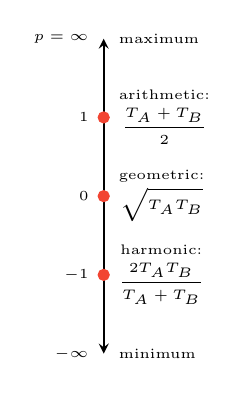
\begin{tikzpicture}
                \tiny
                \tikz[remember picture] \node[coordinate, left=5pt, above=5pt] (d2) {};
                \draw[semithick, <->, >=stealth] (0,0) -- (0,-4);
                \foreach \y in {-1,-2,-3} \draw[semithick] (-2pt, \y cm) -- (2pt, \y cm);
                \draw (0,0) node[left=3pt] {$p=\infty$} node[right=3pt] {maximum};
                \draw (0,-1) node[left=3pt] {$1$} node[right=3pt, align=center] {
                    arithmetic:\\[1ex] $\displaystyle \frac{T_A+T_B}{2}$};
                \draw (0,-2) node[left=3pt] {$0$} node[right=3pt, align=center] {
                    geometric:\\[.4ex] $\displaystyle \sqrt{T_A T_B}$};
                \draw (0,-3) node[left=3pt] {$-1$} node[right=3pt, align=center] {
                    harmonic:\\[1ex] $\displaystyle \frac{2 T_A T_B}{T_A + T_B}$};
                \draw (0,-4) node[left=3pt] {$-\infty$} node[right=3pt] {minimum};
                \draw<2>[pyred, fill=pyred] (0,-1) circle (2 pt);
                \draw<3>[pyred, fill=pyred] (0,-2) circle (2 pt);
                \draw<4>[pyred, fill=pyred] (0,-3) circle (2 pt);
            \end{tikzpicture} 
        \end{column}
    \end{columns}

    \begin{tikzpicture}[remember picture, overlay]
        \path[->, >=stealth, theme] (d1) edge [out=-45, in=45] (d2);
    \end{tikzpicture}
\end{frame}


\begin{frame}{\trento\ initial condition model \quad{\color{almostblack} \scriptsize Phys.\ Rev.\ C 
              {\bf 92}, 011901 (2015)}}
    
    \centering \bigskip \includegraphics{schematic}
    \begin{enumerate}
        \scriptsize \itemsep0.8pt
        \setbeamercolor{item projected}{bg=theme!40, fg=almostblack}
        \item Calc participants: $\displaystyle P_\text{coll}(b) = 
              1 - \exp[-\sigma_{gg} T_{pp}(b)]$, \quad $\displaystyle 
              \int 2 \pi\, b\, db\, P_\text{coll}(b) = 
              \sigma_\text{NN}^\text{inel}$ \\ \vspace{0.1 cm}
        \item Build participant density: $\displaystyle T_A(x,y) = 
              \sum\limits_{i=1}^{N_{\text{part},A}} \gamma_i 
              T_p(x-x_i, y-y_i)$, \quad $\displaystyle \gamma \sim 
              \Gamma(k, 1/k)$
        \item Parametrize entropy deposition: 
              $\displaystyle dS/dy \propto \bigg(\frac{T_A^p + T_B^p}{2} 
              \bigg)^{1/p}$
    \end{enumerate}
\end{frame}


\usebackgroundtemplate{%
\tikz[overlay,remember picture] \node[at=(current page.center)] {
   \includegraphics[width=\paperwidth]{trento_minbias}};
}

\begin{frame}[plain]
\end{frame}

\usebackgroundtemplate{}


\begin{frame}{Compare parametrization to existing IC models}
    \medskip
    \begin{columns}[T]
        \begin{column}{0.03\textwidth}
        \end{column}
        \begin{column}{0.36\textwidth}
            \includegraphics{cgc_compare}
        \end{column}
        \begin{column}{0.01\textwidth}
        \end{column}
        \begin{column}{0.58\textwidth}
            \begin{itemize}
                \smallskip
                \itemsep2ex \small
                \item Wounded nucleon model \\[1em]
                      $\displaystyle \frac{dS}{dy\,d^2r_\perp} 
                      \propto T_A + T_B$ \\[1em]
                      {\scriptsize $^*T$ denotes \emph{participant} thickness} 
                \item EKRT model \; {\scriptsize \color{theme} 
                      PRC 93, 024907 (2016)} \\
                      {\scriptsize after brief free streaming phase} \\[1em] 
                      $\displaystyle \frac{dE_T}{dy\,d^2r_\perp}  \sim 
                      \frac{K_\text{sat}}{\pi} p_\text{sat}^3(K_\text{sat}, 
                      \beta; T_A, T_B)$
                \item KLN model \; {\scriptsize \color{theme} PRC 75, 
                     034905 (2007)} \\[1em] $\displaystyle 
                     \frac{dN_g}{dy\,d^2r_\perp} \sim Q^2_{s,\text{min}} \bigg[2 + 
                     \log \bigg(\frac{Q^2_{s,\text{max}}}{Q^2_{s,\text{min}}}
                     \bigg) \bigg]$
            \end{itemize}
            \centering
        \end{column}
        \begin{column}{0.02\textwidth}
        \end{column}
    \end{columns}
\end{frame}


\begin{frame}{Modern event-by-event hybrid model}
    \bigskip
    \begin{itemize}
        \item \trento\ initial conditions \\
        {\scriptsize Moreland, Bernhard, Bass, PRC {\bf 92}, 
         no.\ 1, 011901 (2015)} \\
        \begin{table}
            \scriptsize \flushleft
            \begin{tabular}{r l}
                norm & entropy normalization \\ 
                $p$ & entropy deposition parameter \\
                $k$ & proton-proton multiplicity fluctuations \\
                $w$ & Gaussian nucleon width
            \end{tabular}
        \end{table}
        \medskip
        \item HotQCD equation of state \\
        {\scriptsize Bazavov, et.\ al.\ PRD {\bf 90}, 
         094503 (2014)} \\
        \smallskip 
        \item iEBE-VISHNU hydrodynamics \\
        {\scriptsize Shen, Qiu, Song, Bernhard, Bass, Heinz, 
         Comp.\ Phys.\ Comm.\ {\bf 199}, 61 (2016)}  
        \begin{table}
            \scriptsize \flushleft
            \begin{tabular}{r l}
                $\eta/s$ min & shear viscosity minimum \\ 
                $\eta/s$ slope & shear viscosity slope \\
                $\zeta/s$ norm & bulk viscosity normalization \\
                $T_\text{sw}$ & hydro-to-urqmd switching temp
            \end{tabular}
        \end{table}
        \medskip
        \item UrQMD hadronic afterburner \\
        {\scriptsize Bass et.\ al, Prog.\ Part.\ Nucl.\ Phys.\ 
         {\bf 41}, 255 (1998)} \\
        {\scriptsize Bleicher et.\ al, J.\ Phys.\ G {\bf 25}, 
         1859 (1999)}
    \end{itemize}
\end{frame}


\begin{frame}{The challenge of rigorous model-to-data comparison}
    \begin{tikzpicture}[overlay, remember picture]
        \node [anchor=east, left=1cm  of current page.north, yshift=-1.8cm] 
            (t1) {\large Parameter};
        \node [anchor=west, right=1cm of current page.north, yshift=-1.8cm] 
            (t2) {\large Observable};
        \node [anchor=east, left=1cm  of current page.north, yshift=-2.4cm] 
            (a1) {\small shear viscosity};
        \node [anchor=east, left=1cm  of current page.north, yshift=-2.9cm] 
            (a2) {\small bulk viscosity};
        \node [anchor=east, left=1cm  of current page.north, yshift=-3.4cm] 
            (a3) {\small pre-equilibrium flow};
        \node [anchor=east, left=1cm  of current page.north, yshift=-3.9cm] 
            (a4) {\small nucleon width};
        \node [anchor=east, left=1cm  of current page.north, yshift=-4.4cm] 
            (a5) {\small hadronization temp};
        \node [anchor=east, left=1cm  of current page.north, yshift=-4.9cm] 
            (a6) {\small p+p fluctuations};
        \node [anchor=west, right=1cm of current page.north, yshift=-2.4cm] 
            (b1) {\small identified yields};
        \node [anchor=west, right=1cm of current page.north, yshift=-2.9cm] 
            (b2) {\small identified mean $p_T$};
        \node [anchor=west, right=1cm of current page.north, yshift=-3.4cm] 
            (b3) {\small flow cumulants};
        \node [anchor=west, right=1cm of current page.north, yshift=-3.9cm] 
            (b4) {\small mode mixing observables};
        \node [anchor=west, right=1cm of current page.north, yshift=-4.4cm] 
            (b5) {\small event plane decorrelations};
        \node [anchor=west, right=1cm of current page.north, yshift=-4.9cm] 
            (b6) {\small HBT interferometry};

        \draw [almostblack, line width=0.2pt] (a1.east) -- (b1.west);
        \draw [almostblack, line width=0.2pt] (a1.east) -- (b2.west);
        \draw [almostblack, line width=0.2pt] (a1.east) -- (b3.west);
        \draw [almostblack, line width=0.2pt] (a1.east) -- (b4.west);
        \draw [almostblack, line width=0.2pt] (a1.east) -- (b5.west);
        \draw [almostblack, line width=0.2pt] (a1.east) -- (b6.west);
        
        \draw [almostblack, line width=0.2pt] (a2.east) -- (b1.west);
        \draw [almostblack, line width=0.2pt] (a2.east) -- (b2.west);
        \draw [almostblack, line width=0.2pt] (a2.east) -- (b3.west);
        \draw [almostblack, line width=0.2pt] (a2.east) -- (b4.west);
        \draw [almostblack, line width=0.2pt] (a2.east) -- (b5.west);
        \draw [almostblack, line width=0.2pt] (a2.east) -- (b6.west);
        
        \draw [almostblack, line width=0.2pt] (a3.east) -- (b1.west);
        \draw [almostblack, line width=0.2pt] (a3.east) -- (b2.west);
        \draw [almostblack, line width=0.2pt] (a3.east) -- (b3.west);
        \draw [almostblack, line width=0.2pt] (a3.east) -- (b4.west);
        \draw [almostblack, line width=0.2pt] (a3.east) -- (b5.west);
        \draw [almostblack, line width=0.2pt] (a3.east) -- (b6.west);

        \draw [almostblack, line width=0.2pt] (a4.east) -- (b1.west);
        \draw [almostblack, line width=0.2pt] (a4.east) -- (b2.west);
        \draw [almostblack, line width=0.2pt] (a4.east) -- (b3.west);
        \draw [almostblack, line width=0.2pt] (a4.east) -- (b4.west);
        \draw [almostblack, line width=0.2pt] (a4.east) -- (b5.west);
        \draw [almostblack, line width=0.2pt] (a4.east) -- (b6.west);

        \draw [almostblack, line width=0.2pt] (a5.east) -- (b1.west);
        \draw [almostblack, line width=0.2pt] (a5.east) -- (b2.west);
        \draw [almostblack, line width=0.2pt] (a5.east) -- (b3.west);
        \draw [almostblack, line width=0.2pt] (a5.east) -- (b4.west);
        \draw [almostblack, line width=0.2pt] (a5.east) -- (b5.west);
        \draw [almostblack, line width=0.2pt] (a5.east) -- (b6.west);
        
        \draw [almostblack, line width=0.2pt] (a6.east) -- (b1.west);
        \draw [almostblack, line width=0.2pt] (a6.east) -- (b2.west);
        \draw [almostblack, line width=0.2pt] (a6.east) -- (b3.west);
        \draw [almostblack, line width=0.2pt] (a6.east) -- (b4.west);
        \draw [almostblack, line width=0.2pt] (a6.east) -- (b5.west);
        \draw [almostblack, line width=0.2pt] (a6.east) -- (b6.west);
    \end{tikzpicture}
    \vspace{4 cm} \\
    \begin{tcolorbox}[width=\textwidth, colback=theme!10, colframe=theme!0]
        \centering
        \small Testing a single set of parameters requires 
               $\mathcal{O}(10^4)$ hydro events \\
        \small \smallskip ...and evaluating eight different parameters 
               five times each\\ requires $5^8 \times 10^4 \approx 10^9$ 
               hydro events. \bigskip \\
        {\large That's roughly $10^5$ computer \emph{years}!}
    \end{tcolorbox}
\end{frame}


\begin{frame}{Solution: Bayesian methodology}
    \vspace{0.7 cm}
    \includegraphics{flowchart}
\end{frame}


\begin{frame}{Calibrating the model: before and after}
    \medskip
    \includegraphics{observables_plot} \\
    \bigskip
    \begin{itemize}
        \small
        \item Top: run model ($\times 10^4$ events) at each design 
              point ($\times300$ evals)
        \vspace{0.2 cm}
        \item Bottom: emulator predictions for 100 samples from 
              the posterior
    \end{itemize}
\end{frame}


\begin{frame}[plain]
    \begin{columns}
        \begin{column}{1 cm}
            \centering
            \hspace{0.5 cm}
            \rotatebox[origin=c]{90}{
                \scriptsize \only<1>{\color{pyblue}} 
                \only<2->{\color{pyblue!40}} 
                    Calibrated to identified particles
            }
        \end{column}
        \begin{column}{\paperheight}
            \centering \vspace{0.3 cm}\\
            \begin{tikzpicture}
                \only<1>{\node [opacity=1] (post) {
                    \includegraphics{posterior}};}
                \only<2->{\node [opacity=0.3] (post) {
                    \includegraphics{posterior}};}
            \end{tikzpicture}
        \end{column}
        \begin{column}{1 cm}
            \centering
            \rotatebox[origin=c]{-90}{
                \scriptsize \only<1>{\color{pyred}} 
                \only<2->{\color{pyred!40}} 
                    Calibrated to charged particles
            }
            \hspace{0.4 cm}
        \end{column}
    \end{columns}

    \only<2>{
    \begin{tikzpicture}[remember picture, overlay]
        \filldraw [draw=almostblack, fill=almostblack, overlay, 
                   opacity=0.1, anchor=center] (current page.south west) 
                   rectangle (\pagewidth,\pagewidth);
        \node[inner sep=0pt, yshift=1cm, overlay] (node1) at 
              (current page.center) {\includegraphics{posterior_p_arrows}};
        \node[inner sep=0pt, below=2ex of node1.south, anchor=north] {
            \begin{tcolorbox}[width=0.552\textwidth, boxrule=0pt, 
                              colback=white, colframe=almostblack, sharp corners]
                \scriptsize \centering
                Generalized mean parametrization: \medskip \\
                $dS/dy \propto \Big(\frac{T_A^p + T_B^p}{2}\Big)^{1/p}$
            \end{tcolorbox}
        };
    \end{tikzpicture}}

    \only<3>{
    \begin{tikzpicture}[remember picture, overlay]
        \filldraw [draw=almostblack, fill=almostblack, overlay, 
            opacity=0.1, anchor=center] (current page.south west) 
            rectangle (\pagewidth,\pagewidth);
        \node[inner sep=0pt, yshift=1cm, overlay] at 
            (current page.center) {\includegraphics{posterior_k}};
        \node[inner sep=0pt, below=2ex of node1.south, anchor=north] {
            \begin{tcolorbox}[width=0.552\textwidth, boxrule=0pt, 
                colback=white, colframe=almostblack, sharp corners]
                \scriptsize \centering
                Random Gamma nucleon weights: \medskip \\
                $P(\gamma\, \vert\, k) = \frac{k^k}{\Gamma(k)} 
                \gamma^{k - 1} e^{-k \gamma}$ \\ 
                $T_A(x,y) = \sum\limits_{i=1}^{N_{\text{part},A}} 
                \gamma_i T_p(x-x_i, y-y_i)$
            \end{tcolorbox}
        };
    \end{tikzpicture}}

    \only<4>{
    \begin{tikzpicture}[remember picture, overlay]
        \filldraw [draw=almostblack, fill=almostblack, overlay, 
            opacity=0.1, anchor=center] (current page.south west) 
            rectangle (\pagewidth,\pagewidth);
        \node[inner sep=0pt, yshift=1cm, overlay] at (current page.center) 
            {\includegraphics{posterior_w}};
        \node[inner sep=0pt, below=2ex of node1.south, anchor=north] {
            \begin{tcolorbox}[width=0.552\textwidth, boxrule=0pt, 
                colback=white, colframe=almostblack, sharp corners]
                \scriptsize \centering
                Gaussian nucleon thickness: \medskip \\
                $T_p(x,y) = \frac{1}{2 \pi w^2} e^{-(x^2 +y^2)/(2w^2)}$
            \end{tcolorbox}
        };
    \end{tikzpicture}}

    \only<5>{
    \begin{tikzpicture}[remember picture, overlay]
        \filldraw [draw=almostblack, fill=almostblack, 
                    overlay, opacity=0.1, 
            anchor=center] (current page.south west) rectangle 
            (\pagewidth,\pagewidth);
        \node[inner sep=0pt, yshift=1cm] at (current page.center) 
            {\includegraphics{etas_estimate}};
        \node[inner sep=0pt, below=2ex of node1.south, anchor=north] {
            \begin{tcolorbox}[width=0.552\textwidth, boxrule=0pt, 
                colback=white, colframe=almostblack, sharp corners]
                \scriptsize \centering
                Shear viscosity parametrization: \medskip \\
                $(\eta/s)(T) = (\eta/s)_\text{min} + (T - T_c) 
                (\eta/s)_\text{slope}$ 
            \end{tcolorbox}
        };
    \end{tikzpicture}}
    
\end{frame}

\begin{frame}{Running the model with high probability parameters}
    \vfill
    \centering
    \begin{columns}
        \begin{column}{0.4\textwidth}
            \scriptsize
            \begin{itemize}
                \item Choose high probability model parameters 
                      from Bayesian posterior (right)
                \smallskip
                \item Run full hybrid model using high probability 
                      parameters (bottom)
            \end{itemize}
        \end{column}
        \begin{column}{0.6\textwidth}
            \scriptsize
            \begin{tabular}{lllll}
                \multicolumn{2}{c}{Initial condition} & & 
                    \multicolumn{2}{c}{QGP medium} \\
                \noalign{\smallskip}\hline\noalign{\medskip}
                norm & 120.          &&  $\eta/s$ min   & 0.08       \\
                $p$  & 0.0           &&  $\eta/s$ slope & 0.85 GeV$^{-1}$   \\
                $k$  & 1.5           &&  $\zeta/s$ norm & 1.25       \\
                $w$  & 0.43 fm       &&  $T_\text{sw}$  & 0.148 GeV  \\
            \end{tabular}
        \end{column}
    \end{columns}
    \vspace{0.5 cm}
    \includegraphics{mode_observables}
\end{frame}

\begin{frame}[plain]{Conclusions}
\medskip
Initial condition properties
\begin{itemize}
    \item Yields, mean $p_T$ and flows impose strong constraints on IC. \\
    \item Entropy  deposition mimicked by $dS/dy \sim \sqrt{T_A T_B}$ \\
    \item Data strongly prefers small nucleon width $w \approx {}$0.4--0.6 fm! \\
    \item A+A collisions weakly sensitive to p+p mult.\ fluctuations \\
    \item Preferred initial conditions similar to EKRT, IP-Glasma \\
\end{itemize}
\smallskip
Hydrodynamic transport properties
\begin{itemize}
    \item First quantitative credibility interval on $(\eta/s)(T)$!
    \item Data prefer non-zero bulk viscosity
    \item Hydro-to-micro $T_\text{sw}$ determined by relative species yields 
\end{itemize}
\medskip \centering
\trento\ is publicly available at \textcolor{pyblue}{\url{qcd.phy.duke.edu/trento}} \\
\medskip More in the pre-print \textcolor{pyblue}{\url{arXiv:1605.03954}}
\end{frame}

\appendix

\begin{frame}{Computer experiment design}
    \begin{columns}
    \begin{column}{0.52\textwidth} 
        Maximin Latin hypercube
        \begin{itemize}
            \item Random, space-filling points
            \item \emph{Maximizes} the \emph{minimum}\\
                distance between points\\
                $\rightarrow$ avoids gaps and clusters
            \item Uniform projections into\\
                lower dimensions
        \end{itemize}
        \medskip
        This work:
        \begin{itemize}
            \item 300 points across 8\\
                dimensions
            \item 8 centrality bins
            \item $\mathcal{O}(10^7)$ events total
        \end{itemize}
    \end{column}
    \begin{column}{0.48\textwidth} 
        \includegraphics[width=\textwidth]{design}
    \end{column}
    \end{columns}
\end{frame}

\begin{frame}[plain]{\trento\ 3D, work in progress...}
    \medskip
    \begin{itemize}
        \scriptsize
        \item Extend to forward/backward rapidities while maintaining mid-rapidity result:\\ 
            \begin{center}
                $s(x_\perp, \eta) = s(x_\perp, \eta=0) \cdot f(x_\perp, \eta)$
            \end{center}
        \item Parametrize $f(x_\perp, \eta)$ by first few cumulants,
            \begin{center}
                \begin{tabular}{cccc}
                    \hline
                    mean & std & skewness & kurtosis \\
                    \hline
                    $\mu(x_\perp)$ & $\sigma(x_\perp)$ & $\gamma(x_\perp)$ & $\kappa(x_\perp)$
                \end{tabular}
            \end{center}
        \item Reconstruct $f(\eta)$ by $\mathcal{F}^{-1}$ cumulant generating function,\\
            \begin{center}
                $\mathcal{F}^{-1} \exp(i\mu k - \frac{\sigma^2}{2} k^2 + i \gamma k^3 - \kappa k^4)$
            \end{center}
    \end{itemize}
    \vfill
    \only<1>{\includegraphics{trento3d_PbPb}}
    \only<2>{\includegraphics{trento3d_pPb}}
    \begin{textblock}{1}(2.5,7.75)
        \only<1>{Pb+Pb}
        \only<2>{p+Pb}
    \end{textblock}
\end{frame}

\begin{frame}{Comparing to the IP-Glasma model}
    \centering
    \begin{columns}
        \begin{column}{0.6\textwidth}
            \includegraphics[width=\textwidth]{ipglasma}
        \end{column}
        \begin{column}{0.4\textwidth}
            \begin{itemize}
                \item IP-Glasma: multi-stage dynamical model, simple analytic mapping unknown.
                \item Analyze effective mapping via eccentricity harmonics $\varepsilon_n$ (left).
            \end{itemize}
        \end{column}
    \end{columns}
    \vspace{0.6cm}
    Work ongoing: determine IP-Glasma effective mapping for direct comparison with \trento\ parametrization
\end{frame}

\begin{frame}{\trento\ charged particle production}
    \centering \bigskip
    \includegraphics[width=0.6\textwidth]{nch_per_npart}
    \begin{itemize}
        \item Entropy deposition parameter $p=0$, nucleon width $w=0.5$~fm, p+p fluctuation factor $k=1.6$, normalization varied with energy but not collision system
        \item Good description of particle production at all energies, self consistent p+A and A+A multiplicities
    \end{itemize}
\end{frame}
\end{document}
